%\hypertarget{___gatsby}{}
%\hypertarget{gatsby-focus-wrapper}{}
%\href{https://mukulrathi.com/}{}
%
%MUKUL RATHI
%
%\href{https://mukulrathi.com/about-me}{}
%
%About Me
%
%\href{https://mukulrathi.com/blog}{}
%
%Blog
%
%\hypertarget{creating-the-bolt-compiler-part-6}{%
%\subsection{Creating the Bolt Compiler: Part
%6}\label{creating-the-bolt-compiler-part-6}}

\hypertarget{top-of-page}{%
\chapter{Desugaring - taking our high-level language and simplifying
it!}\label{top-of-page}}

July 01, 2020

%\hypertarget{july-01-2020}{%
%\subsection{July 01, 2020}\label{july-01-2020}}
%
%\hypertarget{min-read}{%
%\subsection{6 min read}\label{min-read}}

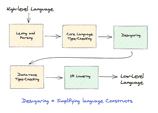
\includegraphics[width=\linewidth]{06_files/desugaring.png}

%\hypertarget{series-creating-the-bolt-compiler}{%
%\section{Series: Creating the Bolt
%Compiler}\label{series-creating-the-bolt-compiler}}
%
%\begin{itemize}
%\item
%  { Part 1:
%  }\href{https://mukulrathi.com/create-your-own-programming-language/intro-to-compiler/}{How
%  I wrote my own "proper" programming language}
%\item
%  { Part 2:
%  }\href{https://mukulrathi.com/create-your-own-programming-language/compiler-engineering-structure/}{So
%  how do you structure a compiler project?}
%\item
%  { Part 3:
%  }\href{https://mukulrathi.com/create-your-own-programming-language/parsing-ocamllex-menhir/}{Writing
%  a Lexer and Parser using OCamllex and Menhir}
%\item
%  { Part 4:
%  }\href{https://mukulrathi.com/create-your-own-programming-language/intro-to-type-checking/}{An
%  accessible introduction to type theory and implementing a
%  type-checker}
%\item
%  { Part 5:
%  }\href{https://mukulrathi.com/create-your-own-programming-language/data-race-dataflow-analysis/}{A
%  tutorial on liveness and alias dataflow analysis}
%\item
%  \textbf{Part 6: Desugaring - taking our high-level language and
%  simplifying it!}
%\item
%  { Part 7:
%  }\href{https://mukulrathi.com/create-your-own-programming-language/protobuf-ocaml-cpp-tutorial/}{A
%  Protobuf tutorial for OCaml and C++}
%\item
%  { Part 8:
%  }\href{https://mukulrathi.com/create-your-own-programming-language/llvm-ir-cpp-api-tutorial/}{A
%  Complete Guide to LLVM for Programming Language Creators}
%\item
%  { Part 9:
%  }\href{https://mukulrathi.com/create-your-own-programming-language/concurrency-runtime-language-tutorial/}{Implementing
%  Concurrency and our Runtime Library}
%\item
%  { Part 10:
%  }\href{https://mukulrathi.com/create-your-own-programming-language/generics-parametric-polymorphism/}{Generics
%  - adding polymorphism to Bolt}
%\item
%  { Part 11:
%  }\href{https://mukulrathi.com/create-your-own-programming-language/inheritance-method-overriding-vtable/}{Adding
%  Inheritance and Method Overriding to Our Language}
%\end{itemize}
%
%\begin{center}\rule{0.5\linewidth}{0.5pt}\end{center}

\hypertarget{just-give-me-the-code}{%
\section{\texorpdfstring{\protect\hyperlink{just-give-me-the-code}{}Just
give me the
code!}{Just give me the code!}}\label{just-give-me-the-code}}

All the illustrative code snippets in this blog post link to the
respective file in the \href{https://github.com/mukul-rathi/bolt}{Bolt
repository}. There's more code in there than could be covered without
making this post extremely long!

The first half of this post will be looking at the
\href{https://github.com/mukul-rathi/bolt/tree/master/src/frontend/desugaring}{desugaring/
folder} and the second half is covering the
\href{https://github.com/mukul-rathi/bolt/tree/master/src/frontend/ir_gen}{ir\_gen/
folder}.

\hypertarget{what-is-desugaring}{%
\section{\texorpdfstring{\protect\hyperlink{what-is-desugaring}{}What
is desugaring?}{What is desugaring?}}\label{what-is-desugaring}}

Programming languages are a series of abstractions. No one writes
programs by typing in 0s and 1s - it's just not human readable. The
closest we get to the hardware operations is with \textbf{assembly code}
e.g. series of \texttt{add} \texttt{mov} and \texttt{jmp} instructions.

Assembly code is still not really a pleasant programming experience.
Even languages we deem as \emph{low-level} like C / C++ / Rust offer a
host of abstractions over assembly code - things you take for granted
like \texttt{if} statements and \texttt{while} loops.

We call these abstractions \textbf{syntactic sugar} - named because they
make it \emph{sweeter} for programmers to program in that language.

When we're writing a compiler though, we're going the other way - we're
\emph{desugaring} the source code - stripping away higher-level
constructs. We also refer to this as \emph{lowering} the high-level
language constructs.

In this post we'll start by looking at desugaring a for loop. We'll then
look at the ``Desugaring'' and ``IR Lowering'' stages in the Bolt
compiler frontend. This will wrap up our compiler frontend and set us up
to switch to C++ for the compiler backend.

\hypertarget{desugaring-for-loops}{%
\section{\texorpdfstring{\protect\hyperlink{desugaring-for-loops}{}Desugaring
For Loops}{Desugaring For Loops}}\label{desugaring-for-loops}}

The first case we desugar is actually between the parsing and
type-checking phases - desugaring a \texttt{for} loop into a while loop:

{desugar\_for\_loop.bolt}

Copy

\begin{verbatim}
for (let i = 0; i < n; i:=i+1) {  doSomething}
// desugared
let i = 0;while (i < n) {  doSomething;  i:=i+1}
\end{verbatim}

Note we handle this as a special case when type-checking the expression,
however you might imagine if there was more sugar (like \texttt{++i}
instead of \texttt{i:=i+1}) that we might add a full desugaring stage
between the parsed AST and typed AST:

\begin{lstlisting}[language=caml,caption={type\_expr.ml}]
let rec type_expr class_defns function_defns (expr : Parsed_ast.expr) env =
...
| Parsed_ast.For
      (loc, start_expr, cond_expr, step_expr, Parsed_ast.Block (block_loc, loop_expr)) ->
      (* desugar into a while loop *)
      type_block_with_defns
        (Parsed_ast.Block
           ( loc
           , [ start_expr
             ; Parsed_ast.While
                 (loc, cond_expr,
                 Parsed_ast.Block (block_loc, loop_expr @ [step_expr]))
             ] ))
        env
\end{lstlisting}
\hypertarget{desugaring-between-type-checking-stages}{%
\section{\texorpdfstring{\protect\hyperlink{desugaring-between-type-checking-stages}{}Desugaring
between type-checking
stages}{Desugaring between type-checking stages}}\label{desugaring-between-type-checking-stages}}

Desugaring gets its own stage in between the two stages of
type-checking. The data-race type-checking is much more complex than the
traditional type-checking (\texttt{int}, \texttt{bool} etc), so we
simplify the language to \emph{avoid having to consider as many cases}.

\hypertarget{removing-variable-shadowing}{%
\subsection{\texorpdfstring{\protect\hyperlink{removing-variable-shadowing}{}Removing
variable
shadowing}{Removing variable shadowing}}\label{removing-variable-shadowing}}

For example, consider variable shadowing, where we can declare the same
variable name \texttt{x} in nested scopes: Consider the following:

%{variable\_shadowing.bolt}
%
%Copy

\begin{verbatim}
let x = 0;
if (x >= 0) {
  let x = 1;
  let y = x + 1
 // we now refer to the value x=1}
else {
 // we refer to the value x=0 
x := 1
}
\end{verbatim}

Variable shadowing is syntactic sugar - we don't require the programmer
to use unique variable names in nested scopes. It makes the
{alias
liveness analysis previously discussed} much harder. How do we know
which value of x is being aliased? We could track which scope we're in
\emph{orrrr} we could avoid it. It's much easier to deal with once we
give variables unique names:

%{unique\_variable\_names.bolt}
%
%Copy

\begin{verbatim}
let _x0 = 0;
if (_x0 >= 0) {
  let _x1 = 1;
  let y = _x1+ 1
} else { _x0 := 1}
\end{verbatim}

We first create a mapping from old to new variable names. We count the
number of times the variable has been declared so far in outer scopes
and stick that count on the end of the variable name. And to specify
that these are compiler-generated names we prepend them with an
\texttt{\_}, since in Bolt programmers can't define a variable starting
with an \texttt{\_}.

\begin{lstlisting}[language=caml,caption={{remove\_variable\_shadowing.ml}}]
type var_name_map = (Var_name.t * Var_name.t) list

let set_unique_name var_name var_name_map =
  let num_times_var_declared =
    List.length (List.filter ~f:(fun (name, _) -> name = var_name) var_name_map) in
  Var_name.of_string
    (Fmt.str "_%s%d" (Var_name.to_string var_name) num_times_var_declared)
\end{lstlisting}


\hypertarget{desugaring-function--method-overloading}{%
\subsection{\texorpdfstring{\protect\hyperlink{desugaring-function--method-overloading}{}Desugaring
Function / Method
Overloading}{Desugaring Function / Method Overloading}}\label{desugaring-function--method-overloading}}

Function overloading is where we define multiple functions with the
\emph{same} name but \emph{different} parameter types. This is useful if
you want to call a different \texttt{print} method based on the type of
the arguments passed in:

%{function\_overloading.bolt}
%
%Copy

\begin{verbatim}
function void print(Foo x){  ...}
function void print(Bar x){  ...}
function void print(int x){  ...}
\end{verbatim}

Again, this is a nice-to-have construct, but we've got an issue - which
function do we call? We can't tell from the source code, but we can use
the information about the argument types from the previous type-checking
stage.

By desugaring more complex language constructs to simpler language
constructs, we make subsequent stages of the compiler simpler - they
\textbf{do not need to know} about anything that has been desugared.

We encode the type of the parameters in the function application
expression when type-checking it:

\begin{lstlisting}[language=caml,caption={type\_expr.ml}]
| Parsed_ast.FunctionApp (loc, func_name, args_exprs) ->
      type_args type_with_defns args_exprs env
      >>= fun (typed_args_exprs, args_types) ->
      get_matching_function_type class_defns func_name args_types function_defns loc
      >>| fun (param_types, return_type) ->
      ( Typed_ast.FunctionApp (loc, return_type, param_types, func_name, typed_args_exprs)
      , return_type )
\end{lstlisting}

\hypertarget{name-mangling-functions}{%
\paragraph{\texorpdfstring{\protect\hyperlink{name-mangling-functions}{}Name
mangling
functions}{Name mangling functions}}\label{name-mangling-functions}}

Now since each overloaded function has differing parameter types, we can
map the parameter types to a unique string, which we append onto our
function name. We call this process of generating a unique function name
\textbf{name mangling}.

We're going to take the approach used in C++.

For each of the primitive types, we can map them to a unique single
character, whilst for classes we map them to the class name prepended
with its length. We then concatenate all param types together.

Why prepend the length? Consider param types \texttt{(Foo\ x,\ Bar\ y)}
and \texttt{(FooBar\ x)} - both would map to \texttt{FooBar} if we
concatenated their parameter names. Only when we prepend the lengths can
they be distinguished - \texttt{3Foo3Bar} vs \texttt{6FooBar}.
%
%{
%\href{https://github.com/mukul-rathi/bolt/blob/master/src/frontend/desugaring/desugar_overloading.ml}{desugar\_overloading.ml}}
%
%Copy

\begin{lstlisting}[caption={desugar\_overloading.ml},language=caml]
let name_mangle_param_types param_types =
  String.concat
    (List.map
       ~f:(function
         | TEVoid                  -> "v"
         | TEInt                   -> "i"
         | TEBool                  -> "b"
         | TEClass (class_name, _) ->
             let class_name_str = Class_name.to_string class_name in
             Fmt.str "%d%s" (String.length class_name_str) class_name_str)
       param_types)
\end{lstlisting}

%\begin{verbatim}
%let name_mangle_param_types param_types =  String.concat    (List.map       ~f:(function         | TEVoid                  -> "v"         | TEInt                   -> "i"         | TEBool                  -> "b"         | TEClass (class_name, _) ->             let class_name_str = Class_name.to_string class_name in             Fmt.str "%d%s" (String.length class_name_str) class_name_str)       param_types)
%\end{verbatim}

And then to name mangle a method or function, we have the following
code:

\begin{lstlisting}[caption={desugar\_overloading.ml},language=caml]
let name_mangle_overloaded_method meth_name param_types =
  Method_name.of_string
    (Fmt.str "_%s%s"
       (Method_name.to_string meth_name)
       (name_mangle_param_types param_types))
\end{lstlisting}

For example, with this name mangling scheme,
\texttt{testFun(Foo\ x,\ Bar\ y)} maps to
\texttt{\_testFun3Foo3Bar(Foo\ x,\ Bar\ y)}.

If you look at the master branch of the Bolt repo, you'll notice the
desugaring stage also desugars generics. That's a topic that deserves
its own post later in the series!

\hypertarget{lowering-to-ir}{%
\section{\texorpdfstring{\protect\hyperlink{lowering-to-ir}{}Lowering
to IR}{Lowering to IR}}\label{lowering-to-ir}}

Recapping so far, we first looked at desugaring for loops - this occurs
between the parsing and first stage of type-checking. We then looked at
the desugaring stage which sits between the two stages of type-checking.
We now look at IR lowering stage that occurs after type-checking.

IR stands for \emph{intermediate representation} - it is simpler than
the source code, but not quite lowered all the way down to assembly
code.

Our goal with this IR is to \textbf{get close to the LLVM
representation}, to make working with the LLVM API as simple as
possible. We'll also strip away any unnecessary information that we
won't need when running the program.

%\hypertarget{i-make-content-about-my-software-engineering-journey-curated-in-my-newsletter}{%
%\subsection{I make content about my software engineering journey,
%curated in my
%newsletter!}\label{i-make-content-about-my-software-engineering-journey-curated-in-my-newsletter}}
%
%Tips from my time at Cambridge and Facebook, and early access to
%technical tutorials on machine learning, compilers and beyond.
%
%\href{https://newsletter.mukulrathi.com/}{Check out previous issues!}
%
%Email Address
%
%By subscribing, you agree with Revue's
%\href{https://www.getrevue.co/terms}{Terms of Service} and
%\href{https://www.getrevue.co/privacy}{Privacy Policy}.

\hypertarget{lowering-objects-to-structs}{%
\subsection{\texorpdfstring{\protect\hyperlink{lowering-objects-to-structs}{}Lowering
Objects to
Structs}{Lowering Objects to Structs}}\label{lowering-objects-to-structs}}

Classes are an \textbf{abstraction} that group together fields and
methods. LLVM IR doesn't contain classes and objects, only
\textbf{structs}, which are just a group of fields.

{
\href{https://mukulrathi.com/static/a394f0ce0e8ccdc6c4aa56d97ee923b1/7f15f/struct-memory.png}{{}
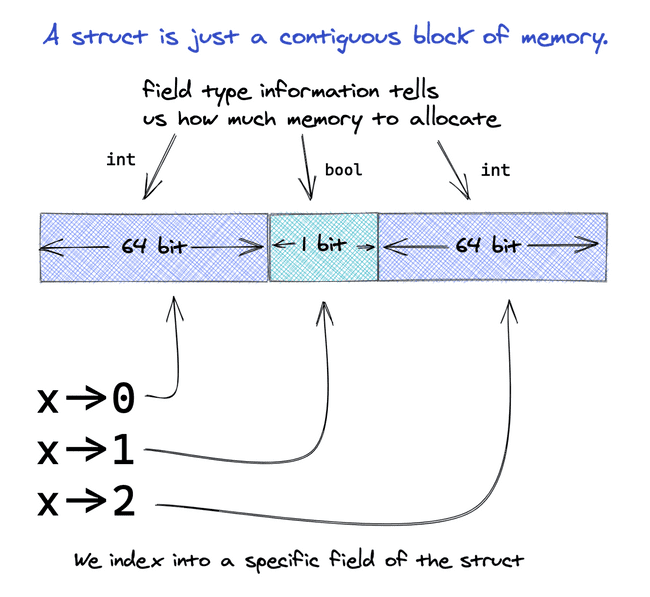
\includegraphics[width=\linewidth]{06_files/struct-memory.png}} }

So how do we map from our Bolt class definition to a struct? We strip
away information from our class:

\begin{itemize}
\tightlist
\item
  We dropped the \texttt{var} / \texttt{const} in the field definitions
\item
  We dropped the capability annotations
\item
  We drop type information in the AST except for field types
\item
  We drop \texttt{loc} (line-position information that we used for our
  type-checker error messages).
\item
  We drop field names
\item
  We no longer associate methods with a class (more on that in a
  second!)
\end{itemize}

Recall, the goal of annotating types and capabilities to our AST is to
check the program is correct. If we can assign a type to an expression,
then it is \emph{well-typed} so it satisfies our notion of correctness.
Likewise, if we can assign capabilities then we know our program doesn't
have data races. And \texttt{const} is just a compiler check to prevent
us reassigning a field.

Once we've checked all that, we can drop that information, since we
don't need it later in the compiler. In fact, our class definition is
now quite barebones - just the class name (a \texttt{string}), and a
list of field types, which LLVM will use to decide how much memory to
allocate to an object:

%{
%\href{https://github.com/mukul-rathi/bolt/blob/master/src/frontend/ir_gen/frontend_ir.mli}{frontend\_ir.mli}}
%
%Copy

\begin{lstlisting}[caption={{frontend\_ir.mli}},language=caml]
type class_defn = TClass of string * type_expr list
\end{lstlisting}

Field names are useful to us as programmers, but for the computer we
don't need to name our fields, we can number them instead as an
\textbf{index} into the struct. Intuitively this is just like array
indices.

%{
%\href{https://github.com/mukul-rathi/bolt/blob/master/src/frontend/ir_gen/ir_gen_env.ml}{ir\_gen\_env.ml}}
%
%Copy

\begin{lstlisting}[caption={{ir\_gen\_env.ml}},language=caml]
let ir_gen_field_index field_name class_name class_defns =
  get_class_fields class_name class_defns
  |> fun field_defns ->
  List.find_mapi_exn
    ~f:(fun index (TField (_, _, name, _)) ->
      if name = field_name then Some index else None)
    field_defns
\end{lstlisting}

%
%\begin{verbatim}
%let ir_gen_field_index field_name class_name class_defns =  get_class_fields class_name class_defns  |> fun field_defns ->  List.find_mapi_exn    ~f:(fun index (TField (_, _, name, _)) ->      if name = field_name then Some index else None)    field_defns
%\end{verbatim}

Note this \texttt{List.find\_mapi\_exn} function name might seem
complex, but the goal is to \texttt{find} the field that matches the
given field name by going through (\texttt{map}) each element of the
list, along with that field's index (hence \texttt{mapi} not
\texttt{map}), and raising an exception (\texttt{exn}) if it is not
found. In practice, this function will never raise an exception because
we already have checked in an earlier type-checking stage that the field
exists.

Methods are just ordinary functions that implicitly take in an
additional parameter: \texttt{this}, which refers to the object that
called the method. In Python, this additional parameter (referred to as
\texttt{self}) is explicitly declared in method declarations.

Note we need to name-mangle our methods again, by prepending the class
name. Right now, we have unique method names \emph{within} a class, when
we separate them as normal functions, they need to be \emph{globally}
uniquely named.

{
\href{https://mukulrathi.com/static/c42e7c83dd7245e132403d79cf89c41e/fa60d/lower-classes.png}{{}
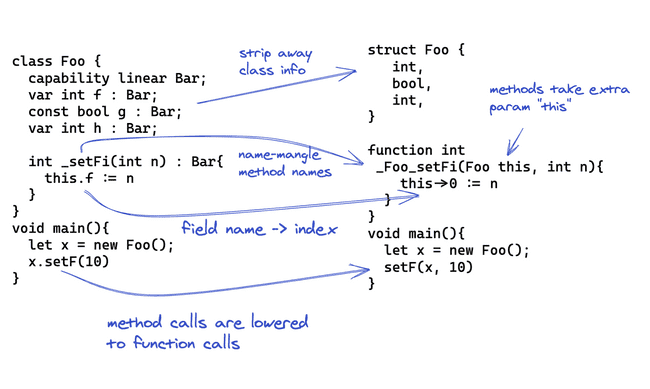
\includegraphics[width=\linewidth]{06_files/lower-classes.png}} }

\hypertarget{automatically-inserting-locks}{%
\subsection{\texorpdfstring{\protect\hyperlink{automatically-inserting-locks}{}Automatically
Inserting
Locks}{Automatically Inserting Locks}}\label{automatically-inserting-locks}}

Bolt has a \texttt{locked} capability, which is similar to the
\texttt{synchronised} keyword in Java - this wraps locks around any
access. Since we're dropping this locked capability we need to specify
lock/unlock instructions in our IR.
%
%{
%\href{https://github.com/mukul-rathi/bolt/blob/master/src/frontend/ir_gen/frontend_ir.mli}{frontend\_ir.mli}}
%
%Copy

\begin{lstlisting}[language=caml,caption={frontend\_ir.mli}]
type lock_type = Reader  | Writer
type expr =  
| Integer     of int  
| Boolean     of bool  
| Identifier  of identifier * lock_type option
  (* maybe acquire a lock when accessing an identifier *) 
 ...  
| Lock        of string * lock_type
  | Unlock    of string * lock_type
\end{lstlisting}

and our to insert locks, we lock the object (\texttt{this}) and then
compute the return value, release the lock and return the value:

%Copy

\begin{verbatim}
... {  methodBody}
// adding locks...
{  lock(this);  
let retVal = methodBody;  
unlock(this);
  retVal}
\end{verbatim}

The corresponding generation code is:

%{
%\href{https://github.com/mukul-rathi/bolt/blob/master/src/frontend/ir_gen/ir_gen_class_and_function_defns.ml}{ir\_gen\_class\_and\_function\_defns.ml}}
%
%Copy

\begin{lstlisting}[language=caml,caption={ir\_gen\_class\_and\_function\_defns.ml}]
let ir_gen_class_method_defn class_defns class_name
    (Desugared_ast.TMethod
       ( method_name
       , _
       (* drop info about whether returning borrowed ref *)
       , return_type
       , params
       , capabilities_used
       , body_expr )) =
    ...
   |> fun ir_body_expr ->
  (* check if we use locked capability *)
  ( match
      List.find
        ~f:(fun (Ast_types.TCapability (mode, _))
        -> mode = Ast_types.Locked)
        capabilities_used
    with
  | Some _lockedCap ->
      [ Frontend_ir.Lock ("this", Frontend_ir.Writer)
      ; Frontend_ir.Let ("retVal", Frontend_ir.Block ir_body_expr)
      ; Frontend_ir.Unlock ("this", Frontend_ir.Writer)
      ; Frontend_ir.Identifier (Frontend_ir.Variable "retVal", None) ]
  | None (* no locks used *) -> ir_body_expr )
  |> fun maybe_locked_ir_body_expr ->
  Frontend_ir.TFunction
    (ir_method_name, ir_return_type, ir_params, maybe_locked_ir_body_expr)
\end{lstlisting}
And for the identifiers, if we're meant to lock them, we acquire a
Reader/Writer Lock depending on whether we're reading from them or
assigning a value to them:

\begin{lstlisting}[language=caml,caption={ir\_gen\_expr.ml}]
let rec ir_gen_expr class_defns expr =
...
  | Desugared_ast.Identifier (_, id) ->
      ir_gen_identifier class_defns id
      |> fun (ir_id, should_lock) ->
      let lock_held = if should_lock then Some Frontend_ir.Reader else None in
      Frontend_ir.Identifier (ir_id, lock_held)
...
  | Desugared_ast.Assign (_, _, id, assigned_expr) ->
      ir_gen_identifier class_defns id
      |> fun (ir_id, should_lock) ->
      ir_gen_expr class_defns assigned_expr
      |> fun ir_assigned_expr ->
      let lock_held = if should_lock then Some Frontend_ir.Writer else None in
      Frontend_ir.Assign (ir_id, ir_assigned_expr, lock_held)
\end{lstlisting}

\hypertarget{wrapping-up-our-compiler-frontend}{%
\section{\texorpdfstring{\protect\hyperlink{wrapping-up-our-compiler-frontend}{}Wrapping
Up Our Compiler
Frontend}{Wrapping Up Our Compiler Frontend}}\label{wrapping-up-our-compiler-frontend}}

As mentioned in the previous parts, the
\href{https://github.com/mukul-rathi/bolt}{Bolt repository} also
contains code for other language features (inheritance and generics,
coming in a later post). So don't worry about ``vtables'' mentioned in
the \texttt{ir\_gen/} folder. To see a simpler version of the repository
before these features were added, run
\texttt{git\ checkout\ simple-compiler-tutorial}.

We've now wrapped up our discussion of the compiler frontend!

Next we're going to be switching from OCaml to C++ for the LLVM IR Code
generation. To do this we'll be using Protobuf, a cross-language binary
serialisation format.

Once we've done that, in a couple of posts we can talk about LLVM's C++
API!

%\hypertarget{share-this-on-twitter}{%
%\subsection{Share This On Twitter}\label{share-this-on-twitter}}
%
%If you liked this post, please consider sharing it with your network. If
%you have any questions, tweet away and I'll answer :) I also tweet when
%new posts drop!
%
%\textbf{PS:} I also share helpful tips and links as I'm learning - so
%you get them \textbf{well before} they make their way into a post!
%
%\hypertarget{series-creating-the-bolt-compiler-1}{%
%\section{Series: Creating the Bolt
%Compiler}\label{series-creating-the-bolt-compiler-1}}
%
%\begin{itemize}
%\item
%  { Part 1:
%  }\href{https://mukulrathi.com/create-your-own-programming-language/intro-to-compiler/}{How
%  I wrote my own "proper" programming language}
%\item
%  { Part 2:
%  }\href{https://mukulrathi.com/create-your-own-programming-language/compiler-engineering-structure/}{So
%  how do you structure a compiler project?}
%\item
%  { Part 3:
%  }\href{https://mukulrathi.com/create-your-own-programming-language/parsing-ocamllex-menhir/}{Writing
%  a Lexer and Parser using OCamllex and Menhir}
%\item
%  { Part 4:
%  }\href{https://mukulrathi.com/create-your-own-programming-language/intro-to-type-checking/}{An
%  accessible introduction to type theory and implementing a
%  type-checker}
%\item
%  { Part 5:
%  }\href{https://mukulrathi.com/create-your-own-programming-language/data-race-dataflow-analysis/}{A
%  tutorial on liveness and alias dataflow analysis}
%\item
%  \textbf{Part 6: Desugaring - taking our high-level language and
%  simplifying it!}
%\item
%  { Part 7:
%  }\href{https://mukulrathi.com/create-your-own-programming-language/protobuf-ocaml-cpp-tutorial/}{A
%  Protobuf tutorial for OCaml and C++}
%\item
%  { Part 8:
%  }\href{https://mukulrathi.com/create-your-own-programming-language/llvm-ir-cpp-api-tutorial/}{A
%  Complete Guide to LLVM for Programming Language Creators}
%\item
%  { Part 9:
%  }\href{https://mukulrathi.com/create-your-own-programming-language/concurrency-runtime-language-tutorial/}{Implementing
%  Concurrency and our Runtime Library}
%\item
%  { Part 10:
%  }\href{https://mukulrathi.com/create-your-own-programming-language/generics-parametric-polymorphism/}{Generics
%  - adding polymorphism to Bolt}
%\item
%  { Part 11:
%  }\href{https://mukulrathi.com/create-your-own-programming-language/inheritance-method-overriding-vtable/}{Adding
%  Inheritance and Method Overriding to Our Language}
%\end{itemize}
%
%\begin{itemize}
%\item ~
%  \hypertarget{a-tutorial-on-liveness-and-alias-dataflow-analysis}{%
%  \subsection{\texorpdfstring{\href{https://mukulrathi.com/create-your-own-programming-language/data-race-dataflow-analysis/}{←
%  A tutorial on liveness and alias dataflow
%  analysis}}{← A tutorial on liveness and alias dataflow analysis}}\label{a-tutorial-on-liveness-and-alias-dataflow-analysis}}
%\item ~
%  \hypertarget{a-protobuf-tutorial-for-ocaml-and-c}{%
%  \subsection{\texorpdfstring{\href{https://mukulrathi.com/create-your-own-programming-language/protobuf-ocaml-cpp-tutorial/}{A
%  Protobuf tutorial for OCaml and C++
%  →}}{A Protobuf tutorial for OCaml and C++ →}}\label{a-protobuf-tutorial-for-ocaml-and-c}}
%\end{itemize}
%
%\hypertarget{table-of-contents}{%
%\section{Table of Contents}\label{table-of-contents}}
%
%\href{https://mukulrathi.com/create-your-own-programming-language/lower-language-constructs-to-llvm/\#top-of-page}{}
%
%\hypertarget{desugaring---taking-our-high-level-language-and-simplifying-it}{%
%\subsection{Desugaring - taking our high-level language and
%simplifying
%it!}\label{desugaring---taking-our-high-level-language-and-simplifying-it}}
%
%\begin{itemize}
%\item
%  \href{https://mukulrathi.com/create-your-own-programming-language/lower-language-constructs-to-llvm/\#just-give-me-the-code}{}
%
%  \hypertarget{just-give-me-the-code-1}{%
%  \subsection{Just give me the code!}\label{just-give-me-the-code-1}}
%\item
%  \href{https://mukulrathi.com/create-your-own-programming-language/lower-language-constructs-to-llvm/\#what-is-desugaring}{}
%
%  \hypertarget{what-is-desugaring-1}{%
%  \subsection{What is desugaring?}\label{what-is-desugaring-1}}
%\item
%  \href{https://mukulrathi.com/create-your-own-programming-language/lower-language-constructs-to-llvm/\#desugaring-for-loops}{}
%
%  \hypertarget{desugaring-for-loops-1}{%
%  \subsection{Desugaring For Loops}\label{desugaring-for-loops-1}}
%\item
%  \href{https://mukulrathi.com/create-your-own-programming-language/lower-language-constructs-to-llvm/\#desugaring-between-type-checking-stages}{}
%
%  \hypertarget{desugaring-between-type-checking-stages-1}{%
%  \subsection{Desugaring between type-checking
%  stages}\label{desugaring-between-type-checking-stages-1}}
%
%  \begin{itemize}
%  \item
%    \href{https://mukulrathi.com/create-your-own-programming-language/lower-language-constructs-to-llvm/\#removing-variable-shadowing}{}
%
%    \hypertarget{removing-variable-shadowing-1}{%
%    \subsection{Removing variable
%    shadowing}\label{removing-variable-shadowing-1}}
%  \item
%    \href{https://mukulrathi.com/create-your-own-programming-language/lower-language-constructs-to-llvm/\#desugaring-function--method-overloading}{}
%
%    \hypertarget{desugaring-function-method-overloading}{%
%    \subsection{Desugaring Function / Method
%    Overloading}\label{desugaring-function-method-overloading}}
%  \end{itemize}
%\item
%  \href{https://mukulrathi.com/create-your-own-programming-language/lower-language-constructs-to-llvm/\#lowering-to-ir}{}
%
%  \hypertarget{lowering-to-ir-1}{%
%  \subsection{Lowering to IR}\label{lowering-to-ir-1}}
%
%  \begin{itemize}
%  \item
%    \href{https://mukulrathi.com/create-your-own-programming-language/lower-language-constructs-to-llvm/\#lowering-objects-to-structs}{}
%
%    \hypertarget{lowering-objects-to-structs-1}{%
%    \subsection{Lowering Objects to
%    Structs}\label{lowering-objects-to-structs-1}}
%  \item
%    \href{https://mukulrathi.com/create-your-own-programming-language/lower-language-constructs-to-llvm/\#automatically-inserting-locks}{}
%
%    \hypertarget{automatically-inserting-locks-1}{%
%    \subsection{Automatically Inserting
%    Locks}\label{automatically-inserting-locks-1}}
%  \end{itemize}
%\item
%  \href{https://mukulrathi.com/create-your-own-programming-language/lower-language-constructs-to-llvm/\#wrapping-up-our-compiler-frontend}{}
%
%  \hypertarget{wrapping-up-our-compiler-frontend-1}{%
%  \subsection{Wrapping Up Our Compiler
%  Frontend}\label{wrapping-up-our-compiler-frontend-1}}
%\end{itemize}
%
%© Mukul Rathi 2023
%
%\hypertarget{gatsby-announcer}{}
%Navigated to Desugaring - taking our high-level language and simplifying
%it!
